\scanpage{20}\mspage{19}
% slanted
\margin{partie de \deleted{\unsure{Th}} \unsure{th.}}
\deleted{\uline{\unsure{Prop}}}\inserted{\uline{Prop} Soit $X,Y$} Deux parties fermées modérées, en pos. rel. modérée. Alors $X\cap Y$ est une partie \inserted{fermée} modérée, et
\[
\boxed{(X\cap Y)^{\cdot}\subset X^{\cdot}\cup Y^{\cdot}}
\]
De plus, \inserted{$X$ et $Y$ ont une borne sup. \unsure{dans|en}} \deleted{parmi \unsure{toutes les} parties} l'ens des parties modérées ordonnées par \deleted{fermées modérées qui \unsure{contient} $X$} l'inclusion.
% slanted
\margin{\deleted{\unsure{D|Dém}} \uline{Dém} double récurrence sur nb de comp. conn. de $X$ et de $Y$ (pour l'existence du Sup et la question des frontières)}
\deleted{$X$ et $Y$, et on} On écrit cette partie $X\underset{\mathrm{mod}}{\cup}Y$, On a
\[
\boxed{(X\underset{\mathrm{mod}}{\cup}Y)^{\cdot}\subset X^{\cdot}\cup Y^{\cdot}}
\]
% slanted
\figure{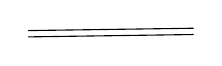
\begin{tikzpicture}[x=1cm,y=1cm]\draw (0,0)--(2.1,0.03);\draw (0,0.08)--(2.1,0.11);\end{tikzpicture}}
\margin{Rem, \unsure{tte} partie modérée $Z$ en pos. rel. \unsure{mod.} avec $X$ et $Y$, l'est aussi avec $X\cap Y$ et $X\underset{\mathrm{mod}}{\cup}Y$}

\uline{Cor} Soit $(X_i)_{i\in I}$ une famille finie de parties fermées modérées mutuellement en pos. \deleted{rel} modérée. Alors $\bigcap_i X_i$ est une partie modérée, et les $X_i$ ont une borne sup. dans l'ens des parties fermées modérées. On a
% slanted
\margin{\uline{Attention} pour une partie \uline{quelc} $A$ de $\mathcal L$, il n'y a \uline{pas} en général d'adh. modérée fermée, i.e. de ``plus petit'' ens f. modéré $X$ tel que $X\supset A$. C'est déjà faux ds le cas standart $L=[0,1]$ ! (Prendre $A=\{0,1/2,1/3\ldots\}$}
\[
\left(\bigcup_{\substack{\mathrm{mod}\\ i}} X_i\right)^{\cdot}\subset\bigcup_i X_i^{\cdot}
\]

\uline{Ex}
\[
[a,b]\underset{\mathrm{mod}}{\cup}[b,c]=[a,c]
\]
mais en général
\[
[a,b]\cup[b,c]\ne[a,c]
\]
(\unsure{prendre|quand} $a$ plus \unsure{c|e} petit élément, $c$ plus grand élément \deleted{\unsure{et}} \unsure{qqconq} \deleted{\unsure{Et en ce} $\unsure{=}$}, $b$ \deleted{\unsure{est}} comp. à tout \inserted{élément de $\mathcal L$.} Si c'est

% pale vertical watermark
% the paper's watermark (EXTRA STRONG), not his text
